\vfill\null
\pagebreak
{\Huge Computador\\}

{\LARGE do latim \textit{computare}:\\

“calcular, estimar, somar, contar”,\\

{\Large de COM-PUTARE, “junto” + “calcular, avaliar, estimar”.\\}

{\LARGE O computador é uma grande calculadora.}

\vfill
\pagebreak

{\LARGE Mas ele também é ótimo para colocar as coisas em \textbf{ordem}.\\}

{\Large no francês: \textit{\textbf{ordinateur}}
	
{\Large no italiano: \textit{\textbf{ordenatore}} (ordenador)\\
		
	\vfill
	\pagebreak

\begin{center}
	
\includegraphics[height=\textheight]{./IMG/Desktop_computer_clipart_-_Yellow_theme.svg.png}
\end{center}

	\vfill
\pagebreak

\begin{center}
	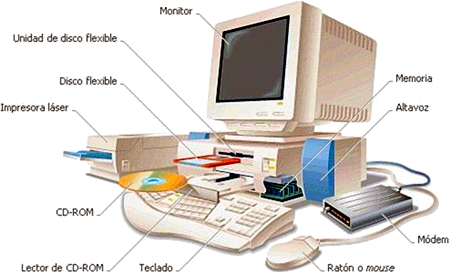
\includegraphics[height=\textheight]{./IMG/th-1517019610.jpg}
\end{center}

\vfill
\pagebreak

\begin{multicols}{3}
	
{\Large Entrada}
	
	\begin{center}
	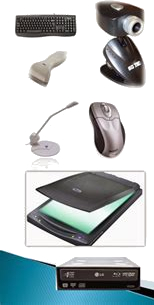
\includegraphics[height=.9\textheight]{./IMG/entrada.jpg}
\end{center}

\vfill
\columnbreak

{\Large Saida}

\begin{center}
	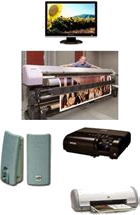
\includegraphics[height=.9\textheight]{./IMG/saida.jpg}
\end{center}

\vfill
\columnbreak

{\Large Mistos}

\begin{center}
	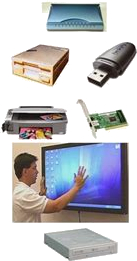
\includegraphics[height=.9\textheight]{./IMG/mistos.jpg}
\end{center}

\vfill
\pagebreak
\end{multicols}

{\large Gabinete ou torre:}
	\begin{center}
		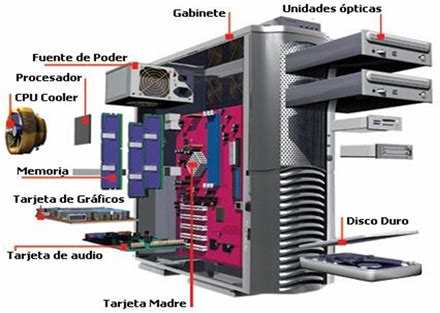
\includegraphics[height=.9\textheight]{./IMG/th-997046030.jpg}
	\end{center}

\vfill
\pagebreak

	\begin{center}
	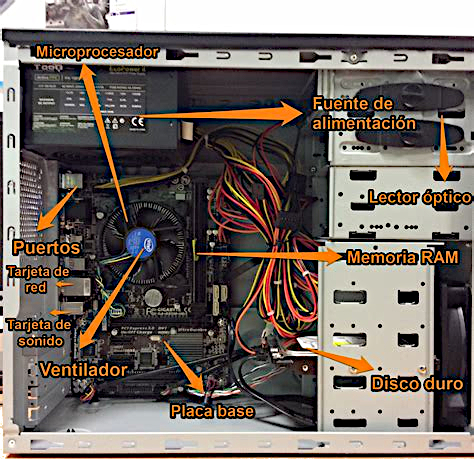
\includegraphics[height=\textheight]{./IMG/th-1583851518.jpg}
\end{center}

\vfill
\pagebreak

\begin{center}
	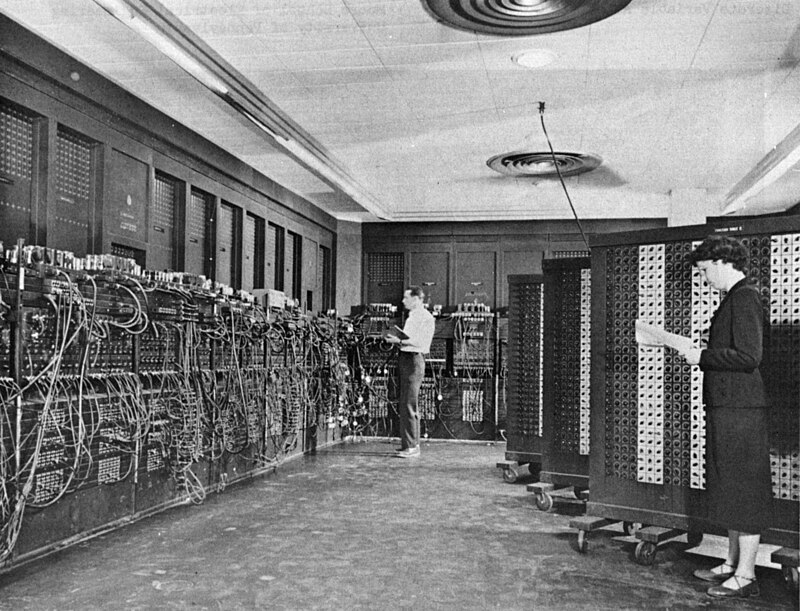
\includegraphics[height=\textheight]{./IMG/ENIAC.jpg}
\end{center}

\vfill
\pagebreak

